\subsection{Ciclo perteneciente}

Información sobre el ciclo al que pertenecen los estudiantes encuestados se muestra en la siguiente tabla.

\begin{multicols}{2}
  \begin{minipage}{\linewidth}
    \centering
	\begin{table}[H]
	  \centering
	  \caption{Distribución por ciclo}
	  \renewcommand{\arraystretch}{1.2}
	  \begin{tabular}{l c c }
		\hline
		Ciclo & \(f_i\) & \(h_i\) \\
		\hline
		1-2 & 60 & \(77.92\%\) \\
		3-4 & 9 & \(11.69\%\) \\
		5-6 & 3 & \(3.90\%\) \\
		7-8 & 2 & \(2.60\%\) \\
		9-10 & 3 & \(3.90\%\) \\
		\hline
		Total & 77 & \(100\%\) \\
		\hline
	  \end{tabular}
	\end{table}
  \end{minipage}

  Se observa que los encuestados pertenecen a los ciclos 1-2, con un 77.92\% del total. Por otro lado, los ciclos 3-4, 5-6, 7-8 y 9-10 representan el 11.69\%, 3.90\%, 2.60\% y 3.90\% respectivamente.

  \columnbreak

  En ese sentido es posible graficar la evidente asimetría de la muestra, para ello se puede calcular el coeficiente de asimetría de Pearson, el cual se define como:
  \begin{equation*}
    A_s = 3 \left( \dfrac{\bar{x} - Me}{s} \right)
  \end{equation*}
  Donde:
  \begin{itemize}
    \item \(\bar{x}\) es la media.
    \item \(Me\) es la mediana.
    \item \(s\) es la desviación estándar.
  \end{itemize}
\end{multicols}
\vspace{-0.5cm}  
  \textbf{Media \(\bar{x}\):}
  \begin{equation*}
    \bar{x} = \dfrac{(1+2)60 + (3+4)9 + (5+6)3 + (7+8)2 + (9+10)3}{77} \approx 15.4
  \end{equation*}
  \textbf{Mediana \(Me\):}
  \begin{equation*}
    Me = \dfrac{77 + 1}{2} = 39
    Me = 1+2 = 3
  \end{equation*}
  \textbf{Desviación estándar \(s\):}
  \begin{equation*}
    s = \sqrt{\dfrac{\sum (x_i - \bar{x})^2}{n}}
    s = \sqrt{\dfrac{(1-15.4)^2(60) + ... + (10-15.4)^2(3)}{77}}
    s \approx 2.07
  \end{equation*}
Sustituyendo los valores en la fórmula, se obtiene:
\begin{equation*}
  A_s = 3 \left( \dfrac{15.4 - 3}{2.07} \right) \approx 20.29
\end{equation*}
El coeficiente de asimetría de Pearson es de aproximadamente 20.29, lo que indica que la distribución de los estudiantes encuestados por ciclo es asimétrica positiva. Esto se debe a que la media es mayor que la mediana, lo que sugiere que la distribución está sesgada hacia la derecha. Por lo tanto, la mayoría de los estudiantes encuestados pertenecen a los ciclos 1-2, lo que explica la asimetría positiva de la distribución.
\textbf{Gráficamente:}
\begin{figure}[H]
	\centering
	\hspace*{-1.5cm}
	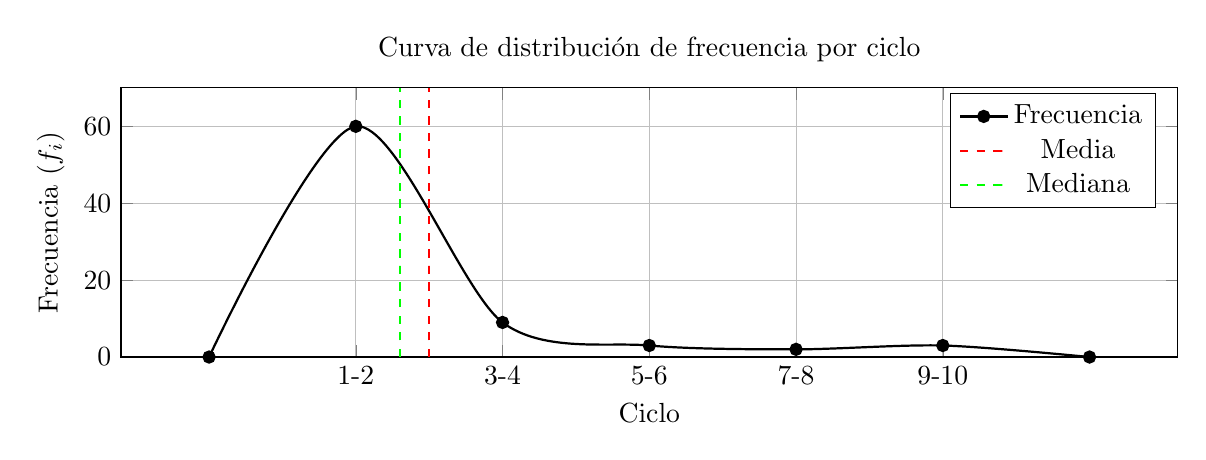
\begin{tikzpicture}
		\begin{axis}[
			width=15cm, height=5cm,
			xlabel={Ciclo},
			ylabel={Frecuencia (\(f_i\))},
			xtick={1, 2, 3, 4, 5},
			xticklabels={1-2, 3-4, 5-6, 7-8, 9-10},
			ymin=0, ymax=70,
			grid=major,
			smooth,
			tension=0.5,
			title={Curva de distribución de frecuencia por ciclo}
			]
			
			% Línea de frecuencia
			\addplot[
			mark=*,
			color=black,
			thick
			] coordinates {
				(0, 0)  % Inicio en 0
				(1, 60) % Ciclo 1-2
				(2, 9)  % Ciclo 3-4
				(3, 3)  % Ciclo 5-6
				(4, 2)  % Ciclo 7-8
				(5, 3)  % Ciclo 9-10
				(6, 0)  % Final en 0
			};
			
			% Media
			\addplot[
			color=red,
			thick,
			dashed
			] coordinates {(1.5, 0) (1.5, 70)}; 
			
			% Mediana
			\addplot[
			color=green,
			thick,
			dashed
			] coordinates {(1.3, 0) (1.3, 70)};
			
			% Agregar leyenda
			\legend{Frecuencia, Media, Mediana}
		\end{axis}
	\end{tikzpicture}
	\caption{Curva de frecuencia por ciclo con medidas de tendencia central}
\end{figure}
